\section{Introduction}

Financial AI systems increasingly turn forecasts, learned signals, policy proposals, and language-model assessments into \emph{weak financial priors}: structured beliefs that may inform an action but do not by themselves confer execution authority. Examples include a language model extracting a directional assessment from an earnings release, a forecast model proposing a position change, or a risk system flagging a credit or liquidity condition. In each case the generator proposes; a separate execution rule decides whether to execute, reduce, route to review, or abstain. Existing financial benchmarks primarily evaluate question answering, forecasting, language understanding, or task completion~\cite{chen2021finqa,xie2023pixiu,xie2024finben,wu2023bloomberggpt,yang2023fingpt}. Agent benchmarks extend evaluation to tool use and multi-step interaction~\cite{liu2023agentbench,zhou2023webarena,qin2023toolllm,mialon2023gaia}, but successful prediction or task completion does not establish that a prior deserves execution authority. We therefore benchmark execution rules and the validity of their evaluation, not predictors.

Figure~\ref{fig:overview} gives the running map of the benchmark. In the paper-test operating points, Cost-Aware authorizes 36.7\% of rows and has the lowest NUAR, 0.064, but ALR 0.245. Hard Role Gate authorizes 75.0\% with ALR zero and leads conservative validation hypervolume, but its NUAR is 0.656. Lifecycle has NUAR 0.147, ALR zero, coverage 0.293, and review rate 0.429. No Action receives NUAR \textit{N/A}, not zero. The benchmark therefore exposes a frontier among negative outcomes, lineage integrity, and usable coverage rather than declaring a universal winner.

The validity argument follows four linked threats: NUAR can fall through coverage collapse; current-role metadata can hide lineage laundering; a controlled ranking can fail to transfer across mechanisms or actual-model proposals; and incomplete power or mechanism coverage can make a positive claim undefined. These threats change the evaluation object, so a reproducible low NUAR is not sufficient evidence of valid authorization.

\begin{figure*}[t]
  \centering
  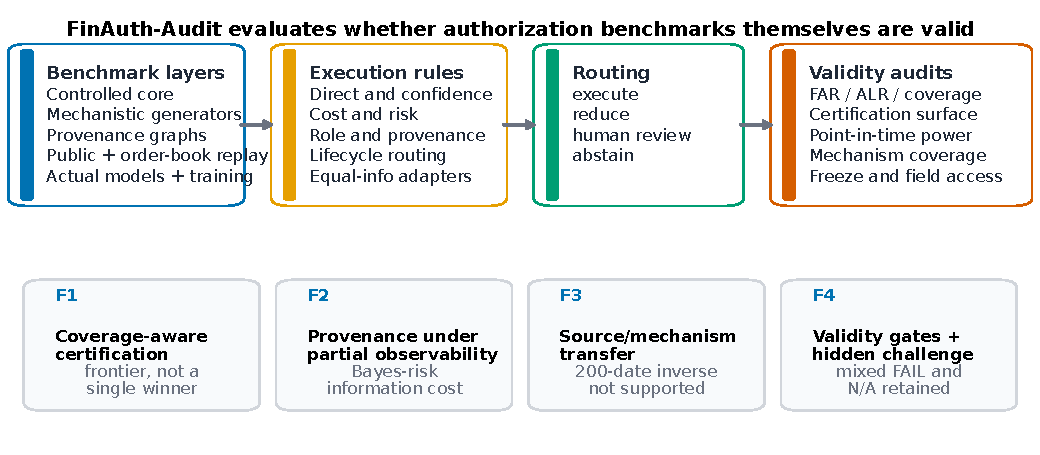
\includegraphics[width=\textwidth]{figures/fig_benchmark_overview.pdf}
  \Description{Flow diagram from benchmark layers through execution rules and four routing decisions to validity audits, followed by four finding boxes for certification, provenance, source transfer, and evidence gates.}
  \caption{\textbf{FinAuth-Audit evaluates whether authorization-benchmark comparisons are valid.} The four stages are benchmark layers, execution rules, routing outcomes, and validity audits. The findings are coverage-aware certification, provenance under partial observability, source and mechanism transfer, and validity gates that retain mixed failures and structural \textit{N/A}.}
  \label{fig:overview}
\end{figure*}

Benchmark outcomes can be fragile to task selection and measurement design~\cite{dehghani2021benchmark,jacobs2021measurement,kiela2021dynabench,ribeiro2020checklist}, while high-stakes data work can accumulate undocumented assumptions and shortcuts~\cite{sambasivan2021data,geirhos2020shortcut,gebru2021datasheets,mitchell2019modelcards}. FinAuth-Audit addresses four coupled blind spots. First, low NUAR can be obtained by suppressing difficult cases. Second, clean current-role metadata can hide upstream lineage laundering. Third, a controlled rule ranking can fail to support its preregistered transfer claim. Fourth, external and training conclusions can be promoted despite insufficient power, collapsed mechanism coverage, or a mixed result.

The benchmark is organized around four linked findings. \textbf{Coverage-aware certification} asks whether NUAR rankings survive joint NUAR, ALR, coverage, utility, and review-load reporting. \textbf{Provenance under partial observability} asks what current roles, full lineage, and missing lineage can identify under delegation, paraphrase, role noise, and multiple hops. \textbf{Transfer validity} asks whether a rule ordering survives mechanism and actual-model shifts. \textbf{Evidence gates} ask whether point-in-time evidence and learned authorization comparisons satisfy predeclared power, effect-size, and mechanism-coverage conditions before positive claims are permitted.

FinAuth-Audit is a benchmark asset and release protocol, not a new execution rule. It contains 124,000 controlled, provenance, and mechanistic event clusters; public event and order-book layers; and a separately frozen 300-date, five-asset, two-task actual-model partition. The latter contains 50 development dates, a one-time 200-date paper test with \RealAgentProposalRows{} cached proposals, and 50 author-unevaluated holdout dates whose proposal plaintext remains encrypted. Latent opportunity, source reliability, costs, stress, and provenance are sampled before rule outputs. Before outcome inspection, existing test clusters were split deterministically into one-time paper tests and community-hidden challenges; evaluators, rules, thresholds, data hashes, and protocols were bound to content-addressed archives.

Our contributions are:
\begin{itemize}
  \item a validity-aware benchmark for execution rules across weak financial priors, with joint coverage, NUAR (legacy artifact field \texttt{FAR}), ALR, utility, missed-opportunity, and review-workload reporting;
  \item branch-neutral utility, sequential-market, and institutional-workflow generators with cluster splits, mechanism holdouts, and a one-time frozen paper/community protocol;
  \item a provenance task with a finite-sample observability limit, direct and indirect laundering, traceable and untraceable delegation, safe-delegation coverage, and structural \textit{N/A}; and
  \item pre-result power, effect-size, and mechanism-coverage gates plus a content-addressed artifact that retains a mixed order-book failure and a larger prospective actual-model test that does not reproduce the inverse rank-transfer pattern observed in a 60-date pilot.
\end{itemize}

EPV serves as one equal-information baseline; removing it does not change any headline conclusion. FinAuth-Audit does not claim deployment readiness, trading profitability, investment advice, public transfer, or a globally optimal rule.
